% Drawing 72/03-3 -- folder 72, batch 03, archive page 48 (PDF page 49).
% Transcription: un segment gradué de $1$ à $n$, le point $k$ marqué
% Kind: graduated segment 1..n. Method 2 (schematic redraw from the facsimile). Status: ok.
% Notes: A segment from 1 to n with the point k marked by a tick; a small dot just right of 1 is drawn as on the page.
% Coordinates: 1 unit = 1 mm = 1/100 of the crop width (bbox in page fractions: [0.12, 0.67, 0.45, 0.715]).
% Redrawn by Claude (claude-opus-5-5), issue #73, 2026-11-07; not checked by a human; not compiled (no TeX in the session).
% Rights: reproduces part of the work -- behind RENDER_TRANSCRIPTS, never published by itself.
\documentclass[tikz,border=3pt]{standalone}
\usepackage{amsmath,amssymb}
\usetikzlibrary{patterns,arrows.meta}
\tikzset{pencil/.style={black!45}, struck/.style={black!35}, mark/.style={circle,draw,inner sep=1.3pt}, pt/.style={circle,fill,inner sep=0.9pt}, opt/.style={circle,draw,fill=white,inner sep=1.1pt}}
\begin{document}
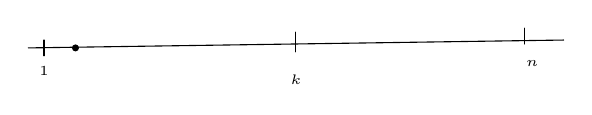
\begin{tikzpicture}[x=1mm,y=1mm,line cap=round,line join=round,font=\scriptsize]
\draw (7,-13) -- (75,-12);
\draw (9,-12) -- (9,-14);
\node[pt] at (13,-13) {};
\draw (41,-11) -- (41,-13.5);
\draw (70,-10.5) -- (70,-12.5);
\node[inner sep=1pt] at (9,-16) {\tiny $1$};
\node[inner sep=1pt] at (41,-17) {\tiny $k$};
\node[inner sep=1pt] at (71,-15) {\tiny $n$};
\end{tikzpicture}
\end{document}
